% Created by tikzDevice version 0.6.2-92-0ad2792 on 2013-03-04 15:02:20
% !TEX encoding = UTF-8 Unicode
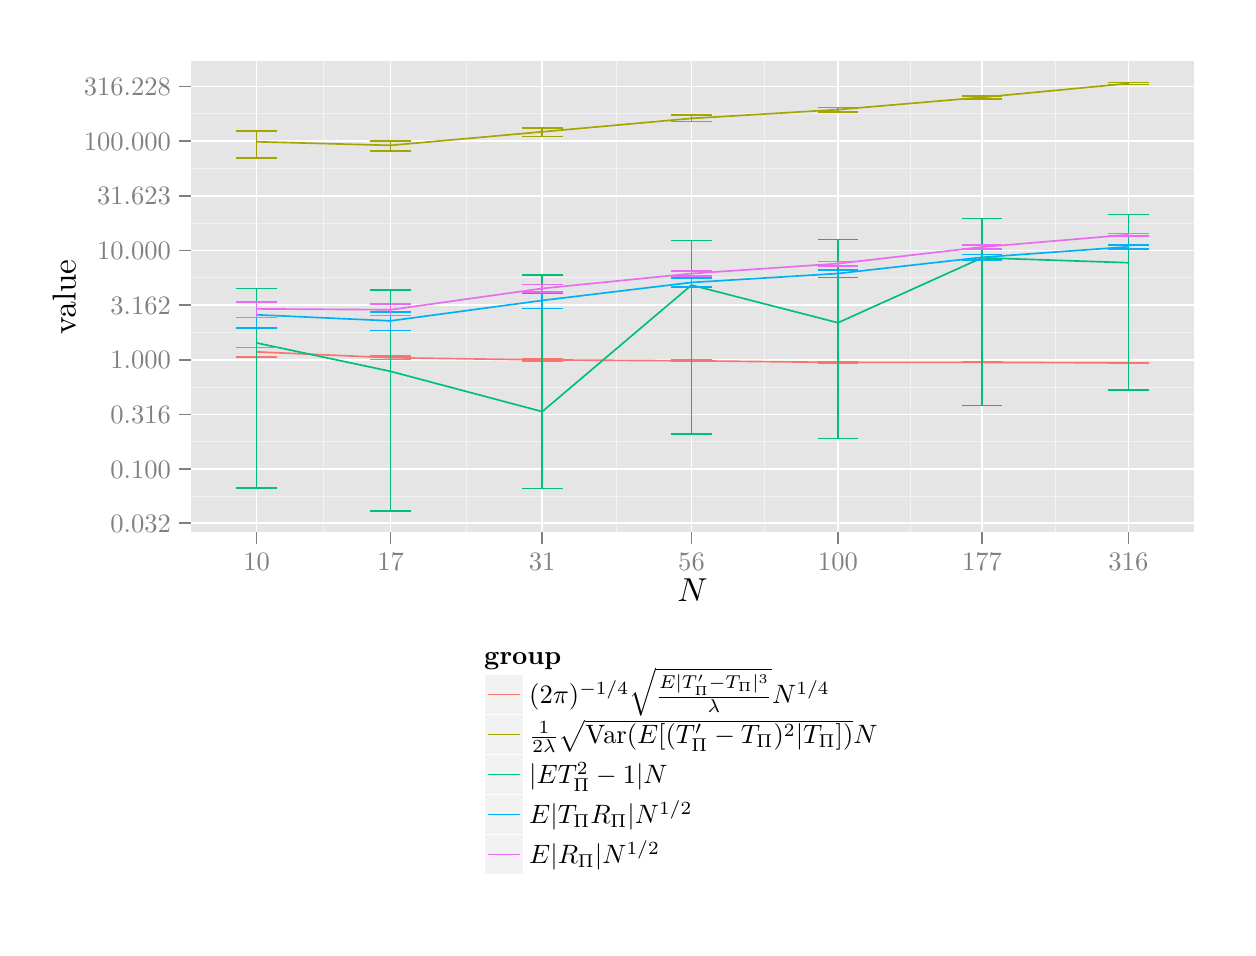
\begin{tikzpicture}[x=1pt,y=1pt]
\definecolor[named]{fillColor}{rgb}{1.00,1.00,1.00}
\path[use as bounding box,fill=fillColor,fill opacity=0.00] (0,0) rectangle (433.62,325.21);
\begin{scope}
\path[clip] (  0.00,  0.00) rectangle (433.62,325.21);
\definecolor[named]{drawColor}{rgb}{1.00,1.00,1.00}
\definecolor[named]{fillColor}{rgb}{1.00,1.00,1.00}

\path[draw=drawColor,line width= 0.6pt,line join=round,line cap=round,fill=fillColor] (  0.00,  0.00) rectangle (433.62,325.21);
\end{scope}
\begin{scope}
\path[clip] ( 58.88,142.81) rectangle (421.57,313.17);
\definecolor[named]{fillColor}{rgb}{0.90,0.90,0.90}

\path[fill=fillColor] ( 58.88,142.81) rectangle (421.57,313.17);
\definecolor[named]{drawColor}{rgb}{0.95,0.95,0.95}

\path[draw=drawColor,line width= 0.3pt,line join=round] ( 58.88,155.94) --
	(421.57,155.94);

\path[draw=drawColor,line width= 0.3pt,line join=round] ( 58.88,175.58) --
	(421.57,175.58);

\path[draw=drawColor,line width= 0.3pt,line join=round] ( 58.88,195.33) --
	(421.57,195.33);

\path[draw=drawColor,line width= 0.3pt,line join=round] ( 58.88,215.08) --
	(421.57,215.08);

\path[draw=drawColor,line width= 0.3pt,line join=round] ( 58.88,234.83) --
	(421.57,234.83);

\path[draw=drawColor,line width= 0.3pt,line join=round] ( 58.88,254.58) --
	(421.57,254.58);

\path[draw=drawColor,line width= 0.3pt,line join=round] ( 58.88,274.33) --
	(421.57,274.33);

\path[draw=drawColor,line width= 0.3pt,line join=round] ( 58.88,294.07) --
	(421.57,294.07);

\path[draw=drawColor,line width= 0.3pt,line join=round] (106.92,142.81) --
	(106.92,313.17);

\path[draw=drawColor,line width= 0.3pt,line join=round] (158.53,142.81) --
	(158.53,313.17);

\path[draw=drawColor,line width= 0.3pt,line join=round] (212.91,142.81) --
	(212.91,313.17);

\path[draw=drawColor,line width= 0.3pt,line join=round] (266.33,142.81) --
	(266.33,313.17);

\path[draw=drawColor,line width= 0.3pt,line join=round] (318.82,142.81) --
	(318.82,313.17);

\path[draw=drawColor,line width= 0.3pt,line join=round] (371.30,142.81) --
	(371.30,313.17);
\definecolor[named]{drawColor}{rgb}{1.00,1.00,1.00}

\path[draw=drawColor,line width= 0.6pt,line join=round] ( 58.88,146.17) --
	(421.57,146.17);

\path[draw=drawColor,line width= 0.6pt,line join=round] ( 58.88,165.71) --
	(421.57,165.71);

\path[draw=drawColor,line width= 0.6pt,line join=round] ( 58.88,185.45) --
	(421.57,185.45);

\path[draw=drawColor,line width= 0.6pt,line join=round] ( 58.88,205.21) --
	(421.57,205.21);

\path[draw=drawColor,line width= 0.6pt,line join=round] ( 58.88,224.96) --
	(421.57,224.96);

\path[draw=drawColor,line width= 0.6pt,line join=round] ( 58.88,244.70) --
	(421.57,244.70);

\path[draw=drawColor,line width= 0.6pt,line join=round] ( 58.88,264.45) --
	(421.57,264.45);

\path[draw=drawColor,line width= 0.6pt,line join=round] ( 58.88,284.20) --
	(421.57,284.20);

\path[draw=drawColor,line width= 0.6pt,line join=round] ( 58.88,303.95) --
	(421.57,303.95);

\path[draw=drawColor,line width= 0.6pt,line join=round] ( 82.72,142.81) --
	( 82.72,313.17);

\path[draw=drawColor,line width= 0.6pt,line join=round] (131.13,142.81) --
	(131.13,313.17);

\path[draw=drawColor,line width= 0.6pt,line join=round] (185.93,142.81) --
	(185.93,313.17);

\path[draw=drawColor,line width= 0.6pt,line join=round] (239.88,142.81) --
	(239.88,313.17);

\path[draw=drawColor,line width= 0.6pt,line join=round] (292.78,142.81) --
	(292.78,313.17);

\path[draw=drawColor,line width= 0.6pt,line join=round] (344.86,142.81) --
	(344.86,313.17);

\path[draw=drawColor,line width= 0.6pt,line join=round] (397.74,142.81) --
	(397.74,313.17);
\definecolor[named]{drawColor}{rgb}{0.97,0.46,0.43}

\path[draw=drawColor,line width= 0.6pt,line join=round] ( 82.72,208.06) --
	(131.13,205.94) --
	(185.93,205.16) --
	(239.88,204.83) --
	(292.78,204.25) --
	(344.86,204.25) --
	(397.74,204.10);
\definecolor[named]{drawColor}{rgb}{0.64,0.65,0.00}

\path[draw=drawColor,line width= 0.6pt,line join=round] ( 82.72,283.98) --
	(131.13,282.68) --
	(185.93,287.58) --
	(239.88,292.42) --
	(292.78,295.60) --
	(344.86,300.03) --
	(397.74,305.03);
\definecolor[named]{drawColor}{rgb}{0.00,0.75,0.49}

\path[draw=drawColor,line width= 0.6pt,line join=round] ( 82.72,211.29) --
	(131.13,201.02) --
	(185.93,186.47) --
	(239.88,232.19) --
	(292.78,218.58) --
	(344.86,242.05) --
	(397.74,240.27);
\definecolor[named]{drawColor}{rgb}{0.00,0.69,0.96}

\path[draw=drawColor,line width= 0.6pt,line join=round] ( 82.72,221.46) --
	(131.13,219.27) --
	(185.93,226.64) --
	(239.88,233.14) --
	(292.78,236.37) --
	(344.86,242.23) --
	(397.74,246.03);
\definecolor[named]{drawColor}{rgb}{0.91,0.42,0.95}

\path[draw=drawColor,line width= 0.6pt,line join=round] ( 82.72,223.59) --
	(131.13,223.27) --
	(185.93,230.97) --
	(239.88,236.36) --
	(292.78,239.96) --
	(344.86,245.93) --
	(397.74,250.40);
\definecolor[named]{drawColor}{rgb}{0.97,0.46,0.43}

\path[draw=drawColor,line width= 0.6pt,line join=round] ( 75.37,209.65) --
	( 90.07,209.65);

\path[draw=drawColor,line width= 0.6pt,line join=round] ( 82.72,209.65) --
	( 82.72,206.30);

\path[draw=drawColor,line width= 0.6pt,line join=round] ( 75.37,206.30) --
	( 90.07,206.30);

\path[draw=drawColor,line width= 0.6pt,line join=round] (123.78,206.65) --
	(138.48,206.65);

\path[draw=drawColor,line width= 0.6pt,line join=round] (131.13,206.65) --
	(131.13,205.27);

\path[draw=drawColor,line width= 0.6pt,line join=round] (123.78,205.27) --
	(138.48,205.27);

\path[draw=drawColor,line width= 0.6pt,line join=round] (178.58,205.53) --
	(193.28,205.53);

\path[draw=drawColor,line width= 0.6pt,line join=round] (185.93,205.53) --
	(185.93,204.79);

\path[draw=drawColor,line width= 0.6pt,line join=round] (178.58,204.79) --
	(193.28,204.79);

\path[draw=drawColor,line width= 0.6pt,line join=round] (232.53,205.05) --
	(247.23,205.05);

\path[draw=drawColor,line width= 0.6pt,line join=round] (239.88,205.05) --
	(239.88,204.61);

\path[draw=drawColor,line width= 0.6pt,line join=round] (232.53,204.61) --
	(247.23,204.61);

\path[draw=drawColor,line width= 0.6pt,line join=round] (285.42,204.35) --
	(300.13,204.35);

\path[draw=drawColor,line width= 0.6pt,line join=round] (292.78,204.35) --
	(292.78,204.13);

\path[draw=drawColor,line width= 0.6pt,line join=round] (285.42,204.13) --
	(300.13,204.13);

\path[draw=drawColor,line width= 0.6pt,line join=round] (337.51,204.31) --
	(352.22,204.31);

\path[draw=drawColor,line width= 0.6pt,line join=round] (344.86,204.31) --
	(344.86,204.19);

\path[draw=drawColor,line width= 0.6pt,line join=round] (337.51,204.19) --
	(352.22,204.19);

\path[draw=drawColor,line width= 0.6pt,line join=round] (390.39,204.13) --
	(405.09,204.13);

\path[draw=drawColor,line width= 0.6pt,line join=round] (397.74,204.13) --
	(397.74,204.06);

\path[draw=drawColor,line width= 0.6pt,line join=round] (390.39,204.06) --
	(405.09,204.06);
\definecolor[named]{drawColor}{rgb}{0.64,0.65,0.00}

\path[draw=drawColor,line width= 0.6pt,line join=round] ( 75.37,287.86) --
	( 90.07,287.86);

\path[draw=drawColor,line width= 0.6pt,line join=round] ( 82.72,287.86) --
	( 82.72,278.15);

\path[draw=drawColor,line width= 0.6pt,line join=round] ( 75.37,278.15) --
	( 90.07,278.15);

\path[draw=drawColor,line width= 0.6pt,line join=round] (123.78,284.15) --
	(138.48,284.15);

\path[draw=drawColor,line width= 0.6pt,line join=round] (131.13,284.15) --
	(131.13,280.71);

\path[draw=drawColor,line width= 0.6pt,line join=round] (123.78,280.71) --
	(138.48,280.71);

\path[draw=drawColor,line width= 0.6pt,line join=round] (178.58,289.06) --
	(193.28,289.06);

\path[draw=drawColor,line width= 0.6pt,line join=round] (185.93,289.06) --
	(185.93,285.85);

\path[draw=drawColor,line width= 0.6pt,line join=round] (178.58,285.85) --
	(193.28,285.85);

\path[draw=drawColor,line width= 0.6pt,line join=round] (232.53,293.55) --
	(247.23,293.55);

\path[draw=drawColor,line width= 0.6pt,line join=round] (239.88,293.55) --
	(239.88,291.29);

\path[draw=drawColor,line width= 0.6pt,line join=round] (232.53,291.29) --
	(247.23,291.29);

\path[draw=drawColor,line width= 0.6pt,line join=round] (285.42,296.39) --
	(300.13,296.39);

\path[draw=drawColor,line width= 0.6pt,line join=round] (292.78,296.39) --
	(292.78,294.74);

\path[draw=drawColor,line width= 0.6pt,line join=round] (285.42,294.74) --
	(300.13,294.74);

\path[draw=drawColor,line width= 0.6pt,line join=round] (337.51,300.58) --
	(352.22,300.58);

\path[draw=drawColor,line width= 0.6pt,line join=round] (344.86,300.58) --
	(344.86,299.47);

\path[draw=drawColor,line width= 0.6pt,line join=round] (337.51,299.47) --
	(352.22,299.47);

\path[draw=drawColor,line width= 0.6pt,line join=round] (390.39,305.43) --
	(405.09,305.43);

\path[draw=drawColor,line width= 0.6pt,line join=round] (397.74,305.43) --
	(397.74,304.62);

\path[draw=drawColor,line width= 0.6pt,line join=round] (390.39,304.62) --
	(405.09,304.62);
\definecolor[named]{drawColor}{rgb}{0.00,0.75,0.49}

\path[draw=drawColor,line width= 0.6pt,line join=round] ( 75.37,230.93) --
	( 90.07,230.93);

\path[draw=drawColor,line width= 0.6pt,line join=round] ( 82.72,230.93) --
	( 82.72,158.86);

\path[draw=drawColor,line width= 0.6pt,line join=round] ( 75.37,158.86) --
	( 90.07,158.86);

\path[draw=drawColor,line width= 0.6pt,line join=round] (123.78,230.43) --
	(138.48,230.43);

\path[draw=drawColor,line width= 0.6pt,line join=round] (131.13,230.43) --
	(131.13,150.56);

\path[draw=drawColor,line width= 0.6pt,line join=round] (123.78,150.56) --
	(138.48,150.56);

\path[draw=drawColor,line width= 0.6pt,line join=round] (178.58,235.90) --
	(193.28,235.90);

\path[draw=drawColor,line width= 0.6pt,line join=round] (185.93,235.90) --
	(185.93,158.68);

\path[draw=drawColor,line width= 0.6pt,line join=round] (178.58,158.68) --
	(193.28,158.68);

\path[draw=drawColor,line width= 0.6pt,line join=round] (232.53,248.32) --
	(247.23,248.32);

\path[draw=drawColor,line width= 0.6pt,line join=round] (239.88,248.32) --
	(239.88,178.34);

\path[draw=drawColor,line width= 0.6pt,line join=round] (232.53,178.34) --
	(247.23,178.34);

\path[draw=drawColor,line width= 0.6pt,line join=round] (285.42,248.65) --
	(300.13,248.65);

\path[draw=drawColor,line width= 0.6pt,line join=round] (292.78,248.65) --
	(292.78,176.77);

\path[draw=drawColor,line width= 0.6pt,line join=round] (285.42,176.77) --
	(300.13,176.77);

\path[draw=drawColor,line width= 0.6pt,line join=round] (337.51,256.29) --
	(352.22,256.29);

\path[draw=drawColor,line width= 0.6pt,line join=round] (344.86,256.29) --
	(344.86,188.72);

\path[draw=drawColor,line width= 0.6pt,line join=round] (337.51,188.72) --
	(352.22,188.72);

\path[draw=drawColor,line width= 0.6pt,line join=round] (390.39,257.65) --
	(405.09,257.65);

\path[draw=drawColor,line width= 0.6pt,line join=round] (397.74,257.65) --
	(397.74,194.34);

\path[draw=drawColor,line width= 0.6pt,line join=round] (390.39,194.34) --
	(405.09,194.34);
\definecolor[named]{drawColor}{rgb}{0.00,0.69,0.96}

\path[draw=drawColor,line width= 0.6pt,line join=round] ( 75.37,225.97) --
	( 90.07,225.97);

\path[draw=drawColor,line width= 0.6pt,line join=round] ( 82.72,225.97) --
	( 82.72,216.72);

\path[draw=drawColor,line width= 0.6pt,line join=round] ( 75.37,216.72) --
	( 90.07,216.72);

\path[draw=drawColor,line width= 0.6pt,line join=round] (123.78,222.44) --
	(138.48,222.44);

\path[draw=drawColor,line width= 0.6pt,line join=round] (131.13,222.44) --
	(131.13,215.74);

\path[draw=drawColor,line width= 0.6pt,line join=round] (123.78,215.74) --
	(138.48,215.74);

\path[draw=drawColor,line width= 0.6pt,line join=round] (178.58,229.17) --
	(193.28,229.17);

\path[draw=drawColor,line width= 0.6pt,line join=round] (185.93,229.17) --
	(185.93,223.72);

\path[draw=drawColor,line width= 0.6pt,line join=round] (178.58,223.72) --
	(193.28,223.72);

\path[draw=drawColor,line width= 0.6pt,line join=round] (232.53,234.80) --
	(247.23,234.80);

\path[draw=drawColor,line width= 0.6pt,line join=round] (239.88,234.80) --
	(239.88,231.45);

\path[draw=drawColor,line width= 0.6pt,line join=round] (232.53,231.45) --
	(247.23,231.45);

\path[draw=drawColor,line width= 0.6pt,line join=round] (285.42,237.70) --
	(300.13,237.70);

\path[draw=drawColor,line width= 0.6pt,line join=round] (292.78,237.70) --
	(292.78,234.96);

\path[draw=drawColor,line width= 0.6pt,line join=round] (285.42,234.96) --
	(300.13,234.96);

\path[draw=drawColor,line width= 0.6pt,line join=round] (337.51,243.25) --
	(352.22,243.25);

\path[draw=drawColor,line width= 0.6pt,line join=round] (344.86,243.25) --
	(344.86,241.27);

\path[draw=drawColor,line width= 0.6pt,line join=round] (337.51,241.27) --
	(352.22,241.27);

\path[draw=drawColor,line width= 0.6pt,line join=round] (390.39,246.75) --
	(405.09,246.75);

\path[draw=drawColor,line width= 0.6pt,line join=round] (397.74,246.75) --
	(397.74,245.28);

\path[draw=drawColor,line width= 0.6pt,line join=round] (390.39,245.28) --
	(405.09,245.28);
\definecolor[named]{drawColor}{rgb}{0.91,0.42,0.95}

\path[draw=drawColor,line width= 0.6pt,line join=round] ( 75.37,226.17) --
	( 90.07,226.17);

\path[draw=drawColor,line width= 0.6pt,line join=round] ( 82.72,226.17) --
	( 82.72,220.44);

\path[draw=drawColor,line width= 0.6pt,line join=round] ( 75.37,220.44) --
	( 90.07,220.44);

\path[draw=drawColor,line width= 0.6pt,line join=round] (123.78,225.36) --
	(138.48,225.36);

\path[draw=drawColor,line width= 0.6pt,line join=round] (131.13,225.36) --
	(131.13,221.19);

\path[draw=drawColor,line width= 0.6pt,line join=round] (123.78,221.19) --
	(138.48,221.19);

\path[draw=drawColor,line width= 0.6pt,line join=round] (178.58,232.39) --
	(193.28,232.39);

\path[draw=drawColor,line width= 0.6pt,line join=round] (185.93,232.39) --
	(185.93,229.59);

\path[draw=drawColor,line width= 0.6pt,line join=round] (178.58,229.59) --
	(193.28,229.59);

\path[draw=drawColor,line width= 0.6pt,line join=round] (232.53,237.33) --
	(247.23,237.33);

\path[draw=drawColor,line width= 0.6pt,line join=round] (239.88,237.33) --
	(239.88,235.36);

\path[draw=drawColor,line width= 0.6pt,line join=round] (232.53,235.36) --
	(247.23,235.36);

\path[draw=drawColor,line width= 0.6pt,line join=round] (285.42,240.75) --
	(300.13,240.75);

\path[draw=drawColor,line width= 0.6pt,line join=round] (292.78,240.75) --
	(292.78,239.19);

\path[draw=drawColor,line width= 0.6pt,line join=round] (285.42,239.19) --
	(300.13,239.19);

\path[draw=drawColor,line width= 0.6pt,line join=round] (337.51,246.57) --
	(352.22,246.57);

\path[draw=drawColor,line width= 0.6pt,line join=round] (344.86,246.57) --
	(344.86,245.29);

\path[draw=drawColor,line width= 0.6pt,line join=round] (337.51,245.29) --
	(352.22,245.29);

\path[draw=drawColor,line width= 0.6pt,line join=round] (390.39,250.83) --
	(405.09,250.83);

\path[draw=drawColor,line width= 0.6pt,line join=round] (397.74,250.83) --
	(397.74,249.95);

\path[draw=drawColor,line width= 0.6pt,line join=round] (390.39,249.95) --
	(405.09,249.95);
\end{scope}
\begin{scope}
\path[clip] (  0.00,  0.00) rectangle (433.62,325.21);
\definecolor[named]{drawColor}{rgb}{0.50,0.50,0.50}

\node[text=drawColor,anchor=base east,inner sep=0pt, outer sep=0pt, scale=  0.96] at ( 51.77,142.86) {0.032};

\node[text=drawColor,anchor=base east,inner sep=0pt, outer sep=0pt, scale=  0.96] at ( 51.77,162.41) {0.100};

\node[text=drawColor,anchor=base east,inner sep=0pt, outer sep=0pt, scale=  0.96] at ( 51.77,182.14) {0.316};

\node[text=drawColor,anchor=base east,inner sep=0pt, outer sep=0pt, scale=  0.96] at ( 51.77,201.90) {1.000};

\node[text=drawColor,anchor=base east,inner sep=0pt, outer sep=0pt, scale=  0.96] at ( 51.77,221.65) {3.162};

\node[text=drawColor,anchor=base east,inner sep=0pt, outer sep=0pt, scale=  0.96] at ( 51.77,241.40) {10.000};

\node[text=drawColor,anchor=base east,inner sep=0pt, outer sep=0pt, scale=  0.96] at ( 51.77,261.15) {31.623};

\node[text=drawColor,anchor=base east,inner sep=0pt, outer sep=0pt, scale=  0.96] at ( 51.77,280.89) {100.000};

\node[text=drawColor,anchor=base east,inner sep=0pt, outer sep=0pt, scale=  0.96] at ( 51.77,300.64) {316.228};
\end{scope}
\begin{scope}
\path[clip] (  0.00,  0.00) rectangle (433.62,325.21);
\definecolor[named]{drawColor}{rgb}{0.50,0.50,0.50}

\path[draw=drawColor,line width= 0.6pt,line join=round] ( 54.61,146.17) --
	( 58.88,146.17);

\path[draw=drawColor,line width= 0.6pt,line join=round] ( 54.61,165.71) --
	( 58.88,165.71);

\path[draw=drawColor,line width= 0.6pt,line join=round] ( 54.61,185.45) --
	( 58.88,185.45);

\path[draw=drawColor,line width= 0.6pt,line join=round] ( 54.61,205.21) --
	( 58.88,205.21);

\path[draw=drawColor,line width= 0.6pt,line join=round] ( 54.61,224.96) --
	( 58.88,224.96);

\path[draw=drawColor,line width= 0.6pt,line join=round] ( 54.61,244.70) --
	( 58.88,244.70);

\path[draw=drawColor,line width= 0.6pt,line join=round] ( 54.61,264.45) --
	( 58.88,264.45);

\path[draw=drawColor,line width= 0.6pt,line join=round] ( 54.61,284.20) --
	( 58.88,284.20);

\path[draw=drawColor,line width= 0.6pt,line join=round] ( 54.61,303.95) --
	( 58.88,303.95);
\end{scope}
\begin{scope}
\path[clip] (  0.00,  0.00) rectangle (433.62,325.21);
\definecolor[named]{drawColor}{rgb}{0.50,0.50,0.50}

\path[draw=drawColor,line width= 0.6pt,line join=round] ( 82.72,138.55) --
	( 82.72,142.81);

\path[draw=drawColor,line width= 0.6pt,line join=round] (131.13,138.55) --
	(131.13,142.81);

\path[draw=drawColor,line width= 0.6pt,line join=round] (185.93,138.55) --
	(185.93,142.81);

\path[draw=drawColor,line width= 0.6pt,line join=round] (239.88,138.55) --
	(239.88,142.81);

\path[draw=drawColor,line width= 0.6pt,line join=round] (292.78,138.55) --
	(292.78,142.81);

\path[draw=drawColor,line width= 0.6pt,line join=round] (344.86,138.55) --
	(344.86,142.81);

\path[draw=drawColor,line width= 0.6pt,line join=round] (397.74,138.55) --
	(397.74,142.81);
\end{scope}
\begin{scope}
\path[clip] (  0.00,  0.00) rectangle (433.62,325.21);
\definecolor[named]{drawColor}{rgb}{0.50,0.50,0.50}

\node[text=drawColor,anchor=base,inner sep=0pt, outer sep=0pt, scale=  0.96] at ( 82.72,129.09) {10};

\node[text=drawColor,anchor=base,inner sep=0pt, outer sep=0pt, scale=  0.96] at (131.13,129.09) {17};

\node[text=drawColor,anchor=base,inner sep=0pt, outer sep=0pt, scale=  0.96] at (185.93,129.09) {31};

\node[text=drawColor,anchor=base,inner sep=0pt, outer sep=0pt, scale=  0.96] at (239.88,129.09) {56};

\node[text=drawColor,anchor=base,inner sep=0pt, outer sep=0pt, scale=  0.96] at (292.78,129.09) {100};

\node[text=drawColor,anchor=base,inner sep=0pt, outer sep=0pt, scale=  0.96] at (344.86,129.09) {177};

\node[text=drawColor,anchor=base,inner sep=0pt, outer sep=0pt, scale=  0.96] at (397.74,129.09) {316};
\end{scope}
\begin{scope}
\path[clip] (  0.00,  0.00) rectangle (433.62,325.21);
\definecolor[named]{drawColor}{rgb}{0.00,0.00,0.00}

\node[text=drawColor,anchor=base,inner sep=0pt, outer sep=0pt, scale=  1.20] at (240.23,117.81) {$N$};
\end{scope}
\begin{scope}
\path[clip] (  0.00,  0.00) rectangle (433.62,325.21);
\definecolor[named]{drawColor}{rgb}{0.00,0.00,0.00}

\node[text=drawColor,rotate= 90.00,anchor=base,inner sep=0pt, outer sep=0pt, scale=  1.20] at ( 17.30,227.99) {value};
\end{scope}
\begin{scope}
\path[clip] (  0.00,  0.00) rectangle (433.62,325.21);
\definecolor[named]{fillColor}{rgb}{1.00,1.00,1.00}

\path[fill=fillColor] (160.71, 14.89) rectangle (319.75,105.93);
\end{scope}
\begin{scope}
\path[clip] (  0.00,  0.00) rectangle (433.62,325.21);
\definecolor[named]{drawColor}{rgb}{0.00,0.00,0.00}

\node[text=drawColor,anchor=base west,inner sep=0pt, outer sep=0pt, scale=  0.96] at (164.98, 95.04) {\bfseries group};
\end{scope}
\begin{scope}
\path[clip] (  0.00,  0.00) rectangle (433.62,325.21);
\definecolor[named]{drawColor}{rgb}{1.00,1.00,1.00}
\definecolor[named]{fillColor}{rgb}{0.95,0.95,0.95}

\path[draw=drawColor,line width= 0.6pt,line join=round,line cap=round,fill=fillColor] (164.98, 76.97) rectangle (179.43, 91.43);
\end{scope}
\begin{scope}
\path[clip] (  0.00,  0.00) rectangle (433.62,325.21);
\definecolor[named]{drawColor}{rgb}{0.97,0.46,0.43}

\path[draw=drawColor,line width= 0.6pt,line join=round] (166.42, 84.20) -- (177.98, 84.20);
\end{scope}
\begin{scope}
\path[clip] (  0.00,  0.00) rectangle (433.62,325.21);
\definecolor[named]{drawColor}{rgb}{0.97,0.46,0.43}

\path[draw=drawColor,line width= 0.6pt,line join=round] (166.42, 84.20) -- (177.98, 84.20);
\end{scope}
\begin{scope}
\path[clip] (  0.00,  0.00) rectangle (433.62,325.21);
\definecolor[named]{drawColor}{rgb}{1.00,1.00,1.00}
\definecolor[named]{fillColor}{rgb}{0.95,0.95,0.95}

\path[draw=drawColor,line width= 0.6pt,line join=round,line cap=round,fill=fillColor] (164.98, 62.52) rectangle (179.43, 76.97);
\end{scope}
\begin{scope}
\path[clip] (  0.00,  0.00) rectangle (433.62,325.21);
\definecolor[named]{drawColor}{rgb}{0.64,0.65,0.00}

\path[draw=drawColor,line width= 0.6pt,line join=round] (166.42, 69.75) -- (177.98, 69.75);
\end{scope}
\begin{scope}
\path[clip] (  0.00,  0.00) rectangle (433.62,325.21);
\definecolor[named]{drawColor}{rgb}{0.64,0.65,0.00}

\path[draw=drawColor,line width= 0.6pt,line join=round] (166.42, 69.75) -- (177.98, 69.75);
\end{scope}
\begin{scope}
\path[clip] (  0.00,  0.00) rectangle (433.62,325.21);
\definecolor[named]{drawColor}{rgb}{1.00,1.00,1.00}
\definecolor[named]{fillColor}{rgb}{0.95,0.95,0.95}

\path[draw=drawColor,line width= 0.6pt,line join=round,line cap=round,fill=fillColor] (164.98, 48.07) rectangle (179.43, 62.52);
\end{scope}
\begin{scope}
\path[clip] (  0.00,  0.00) rectangle (433.62,325.21);
\definecolor[named]{drawColor}{rgb}{0.00,0.75,0.49}

\path[draw=drawColor,line width= 0.6pt,line join=round] (166.42, 55.29) -- (177.98, 55.29);
\end{scope}
\begin{scope}
\path[clip] (  0.00,  0.00) rectangle (433.62,325.21);
\definecolor[named]{drawColor}{rgb}{0.00,0.75,0.49}

\path[draw=drawColor,line width= 0.6pt,line join=round] (166.42, 55.29) -- (177.98, 55.29);
\end{scope}
\begin{scope}
\path[clip] (  0.00,  0.00) rectangle (433.62,325.21);
\definecolor[named]{drawColor}{rgb}{1.00,1.00,1.00}
\definecolor[named]{fillColor}{rgb}{0.95,0.95,0.95}

\path[draw=drawColor,line width= 0.6pt,line join=round,line cap=round,fill=fillColor] (164.98, 33.61) rectangle (179.43, 48.07);
\end{scope}
\begin{scope}
\path[clip] (  0.00,  0.00) rectangle (433.62,325.21);
\definecolor[named]{drawColor}{rgb}{0.00,0.69,0.96}

\path[draw=drawColor,line width= 0.6pt,line join=round] (166.42, 40.84) -- (177.98, 40.84);
\end{scope}
\begin{scope}
\path[clip] (  0.00,  0.00) rectangle (433.62,325.21);
\definecolor[named]{drawColor}{rgb}{0.00,0.69,0.96}

\path[draw=drawColor,line width= 0.6pt,line join=round] (166.42, 40.84) -- (177.98, 40.84);
\end{scope}
\begin{scope}
\path[clip] (  0.00,  0.00) rectangle (433.62,325.21);
\definecolor[named]{drawColor}{rgb}{1.00,1.00,1.00}
\definecolor[named]{fillColor}{rgb}{0.95,0.95,0.95}

\path[draw=drawColor,line width= 0.6pt,line join=round,line cap=round,fill=fillColor] (164.98, 19.16) rectangle (179.43, 33.61);
\end{scope}
\begin{scope}
\path[clip] (  0.00,  0.00) rectangle (433.62,325.21);
\definecolor[named]{drawColor}{rgb}{0.91,0.42,0.95}

\path[draw=drawColor,line width= 0.6pt,line join=round] (166.42, 26.39) -- (177.98, 26.39);
\end{scope}
\begin{scope}
\path[clip] (  0.00,  0.00) rectangle (433.62,325.21);
\definecolor[named]{drawColor}{rgb}{0.91,0.42,0.95}

\path[draw=drawColor,line width= 0.6pt,line join=round] (166.42, 26.39) -- (177.98, 26.39);
\end{scope}
\begin{scope}
\path[clip] (  0.00,  0.00) rectangle (433.62,325.21);
\definecolor[named]{drawColor}{rgb}{0.00,0.00,0.00}

\node[text=drawColor,anchor=base west,inner sep=0pt, outer sep=0pt, scale=  0.96] at (181.24, 80.90) {$(2\pi)^{-1/4}\sqrt{\frac{\mathbb{E}|T'_{\Pi}-T_{\Pi}|^3}{\lambda}}N^{1/4}\quad $};
\end{scope}
\begin{scope}
\path[clip] (  0.00,  0.00) rectangle (433.62,325.21);
\definecolor[named]{drawColor}{rgb}{0.00,0.00,0.00}

\node[text=drawColor,anchor=base west,inner sep=0pt, outer sep=0pt, scale=  0.96] at (181.24, 66.44) {$\frac{1}{2\lambda}\sqrt{\mathrm{Var}(\mathbb{E}[(T'_{\Pi}-T_{\Pi})^2|T_{\Pi}])}N\quad $};
\end{scope}
\begin{scope}
\path[clip] (  0.00,  0.00) rectangle (433.62,325.21);
\definecolor[named]{drawColor}{rgb}{0.00,0.00,0.00}

\node[text=drawColor,anchor=base west,inner sep=0pt, outer sep=0pt, scale=  0.96] at (181.24, 51.99) {$|\mathbb{E}T_{\Pi}^2-1|N\quad $};
\end{scope}
\begin{scope}
\path[clip] (  0.00,  0.00) rectangle (433.62,325.21);
\definecolor[named]{drawColor}{rgb}{0.00,0.00,0.00}

\node[text=drawColor,anchor=base west,inner sep=0pt, outer sep=0pt, scale=  0.96] at (181.24, 37.53) {$\mathbb{E}|T_{\Pi}R_{\Pi}|N^{1/2}\quad $};
\end{scope}
\begin{scope}
\path[clip] (  0.00,  0.00) rectangle (433.62,325.21);
\definecolor[named]{drawColor}{rgb}{0.00,0.00,0.00}

\node[text=drawColor,anchor=base west,inner sep=0pt, outer sep=0pt, scale=  0.96] at (181.24, 23.08) {$\mathbb{E}|R_{\Pi}|N^{1/2}\quad $};
\end{scope}
\end{tikzpicture}
